We face a real-world problem as the last lab.

After understanding the problem and understanding what method use to solve it, we proceed by checking data in the dataset:
\begin{itemize}
	
	\item Categorical features
	\item Missing values
	\item Numerical problems
	
\end{itemize}
We normalize the data so that each feature has the same weight in the solution.
We control the distribution of data, checking the various categorical features that possibly have a Gaussian distribution: the Gaussian distribution indicates that data come from nature.
We observe that during the calculation two types of errors are kept:
\begin{itemize}
	
	\item Error on validation: used to optimize $\gamma$ and $\lambda$
	\item Error on the test: tells me that if we take the data and we do learning with those particular $\gamma$ and $\lambda$, we get a model with that particular unbiased error

	
\end{itemize}
To verify the goodness of model a single parameter is not enough (error for example), then we print a scatter plot: $x$ axis $\rightarrow$ true value, $y$ axis $\rightarrow$ prediction.\\
\textbf{Ideal case}: there is a line, so the values coincide exactly.\\
\textbf{Real case}: there is a bubble, an elipsoid is formed around the straight line
Using more data for learning we can improve prediction quality, so we can try to change percentages.

We note that $\lambda_{best} = 10^{-4}$ and $\gamma_{best} = 2.2122$. $\lambda$ indicates the smoothness of the model and $\gamma$ indicates its non-linearity, but in itself we can not evaluate whether they are large or small.
To evaluate whether the range is large or small we have to evaluate the dimensionality of the space, if we are in a low-dimensional space, $\gamma = 2$ is probably large, while in one of great dimensionality it is probably small. In turn, lambda depends on the cardinality of the space, it happens that if we have small numbers in $\omega$, $\lambda$ will be large and then very regularize the solution.
In this case the size of the space is 11, so $\gamma = 2$ can be considered small.\\
\begin{figure}
We verify the distribution of the data, here for example the first categorical feature (X (:, 1)) the fact that it has a Gaussian distribution is a good sign because it is the correct distribution for data coming from nature:\\
	
	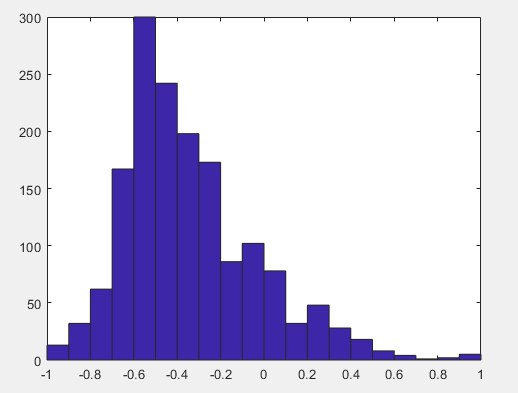
\includegraphics[width=0.5\textwidth]{hist1.png}
	\centering
	\caption{$\lambda$ = 1 $\gamma$ = 1}
	\label{fig:\lambda = 1 \gamma = 1}

	
\end{figure}

\begin{figure}

Solution with $\gamma_{best}$ and $\lambda_{best}$, values that minimize the error\\

	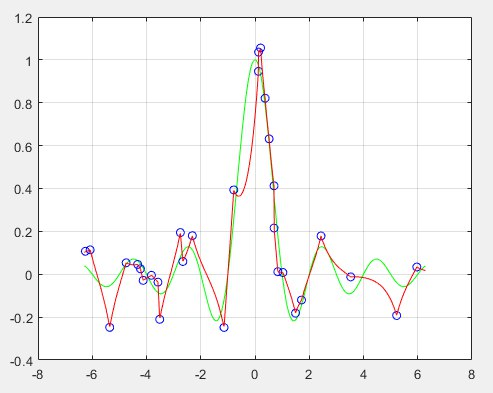
\includegraphics[width=0.5\textwidth]{kmlbgb.png}
	\centering
	\caption{$\lambda$best $\gamma$best}
%	\label{fig:\lambda_best \gamma_best}
	
	
\end{figure}

\begin{figure}
	
	We verify the distribution of data, here for example the first categorical feature (X (:, 1))
	the fact that it has a Gaussian distribution is a good sign because it is the correct distribution for data coming from nature\\
	
	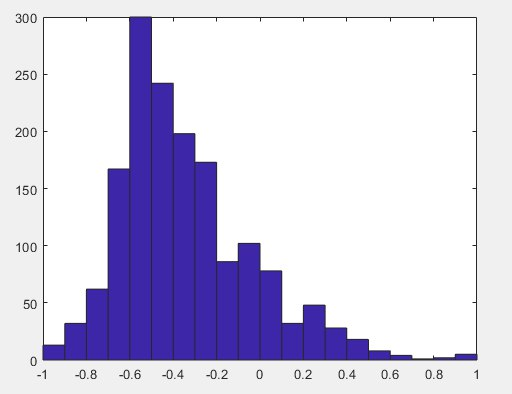
\includegraphics[width=0.5\textwidth]{hist2.png}
	\centering
	\caption{$\lambda$best $\gamma$best}
%	\label{fig:\lambda_best \gamma_best}
	
	
\end{figure}

\begin{figure}
	
	Scatter plot: x axis $\rightarrow$ true value, y axis $\rightarrow$ prediction\\
	
	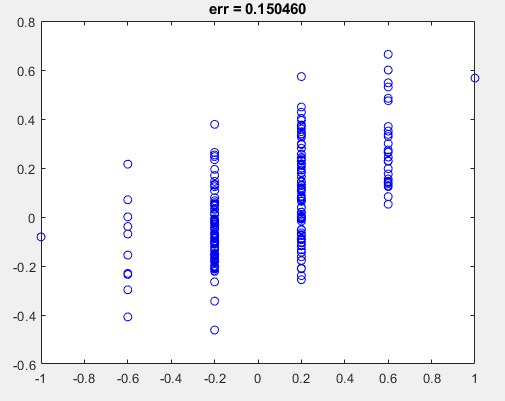
\includegraphics[width=0.5\textwidth]{scatter.png}
	\centering
	\caption{$\lambda$best $\gamma$best}
%	\label{fig:\lambda_best \gamma_best}
	
	
\end{figure}

\begin{figure}
	
	Recalculated with k = 30\\
	
	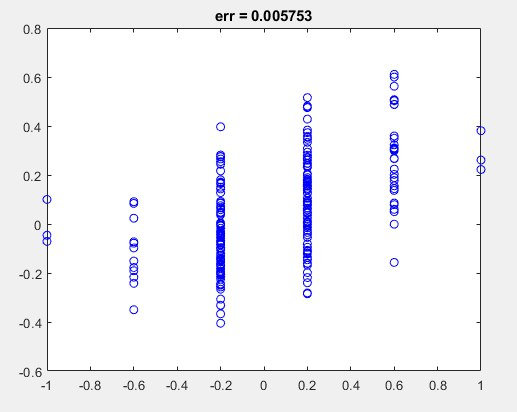
\includegraphics[width=0.5\textwidth]{scatter2.png}
	\centering
	\caption{$\lambda$best $\gamma$best}
%	\label{fig:\lambda_best \gamma_best}
	
	
\end{figure}


